\section{Spektrogram}

Byl zobrazen spektrogram celého signálu pomocí funkce spektrogram z knihovny scipy a také jeho výkonová spektrální hustota. Místo této funkce by šla použít přímo naše fourierova transformace u předchozího kroku použítá na každý frame, ale bylo by zbytečné ji použít když máme k dispozici přímo funkci, která nám vygeneruje rovnou data celého spektrogramu bez nutnosti dalších operací s daty na naší straně. Další výhodou bude rychlost zpracování, protože tato knihovna je velmi optimalizovaná narozdíl od naší implementace. \\
Pro další krok - určení rušivých frekvencí, byl vytvořen i graf výkonové spektrální hustoty pro první frame signálu (pouze šum).

Pro vytvoření spektrogramů bude použita funkce scipy.signal.spectrogram z knihovny scipy, která má jako argumenty signál, vzorkovací frekvenci, velikost rámce a překrytí rámců, takže není potřeba generovat data ručně, protože tato funkce se o to postará i o vytvoření rámců.
Tato funkce vrací pole frekvencí, pole časů a pole výkonové hustoty. Tyto hodnoty jsou poté dobrazeny pomocí plt.pcolormesh.

Pro vytvoření spektrálních hustot bude použita funkce scipy.signal.periodogram z knihovny scipy s argumenty vstupní signál, vzorkovací frekvence a scaling, kde pro scaling byl použit parametr "density".
Tato funkce vrací pole frekvencí a pole hustot.
Tyto hodnoty jsou poté zobrazení pomocí plt.semilogy.

\begin{figure}[H] 
	\centering
	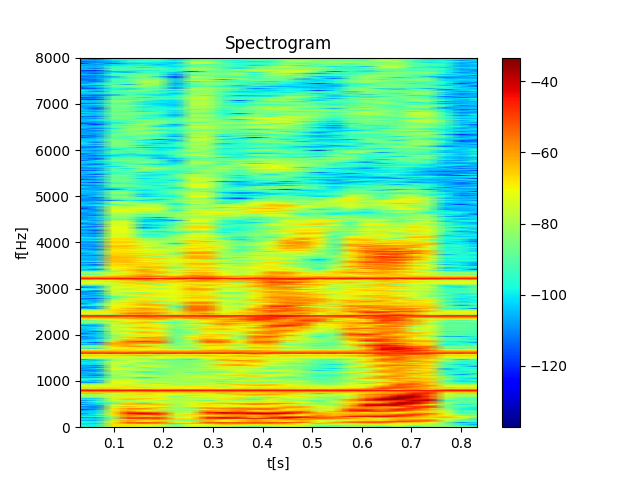
\includegraphics[scale=0.7,keepaspectratio]{Figure_6}
	\caption{Výkonový spektrogram}
\end{figure}

\begin{figure}[H] 
	\centering
	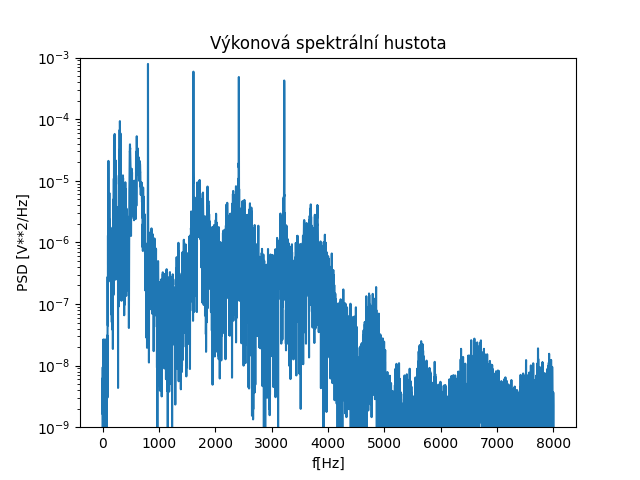
\includegraphics[scale=0.7,keepaspectratio]{Figure_7}
	\caption{Výkonová spektrální hustota}
\end{figure}

\begin{figure}[H] 
	\centering
	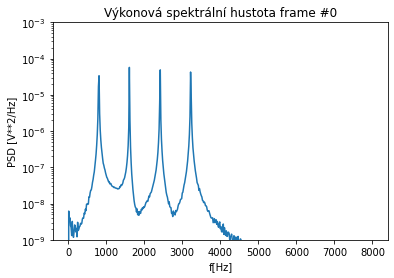
\includegraphics[scale=0.7,keepaspectratio]{Figure_26}
	\caption{Výkonová spektrální hustota frame \#0}
\end{figure}